\begin{spacing}{2}
Aerial Robotic Swarms refer to a group of autonomous unmanned aerial vehicles capable of coordinating and interacting with each other in a shared environment for performing tasks to achieve a common goal.

The idea of UAV swarms has been directly inspired from the flocks of birds travelling together in nature. Birds travelling long distances for migration have been observed to maintain formations which reduce the overall drag on the flock thereby increasing efficiency and saving energy. Travelling in groups also provide benefits like increased navigational accuracy and protection from predators as observed in groups of other animals and insects.
Use of multiple coordinated and cooperative vehicles helps increase reliability, redundancy, area coverage and save time.
\begin{figure}[h]
\begin{subfigure}{0.49\linewidth}
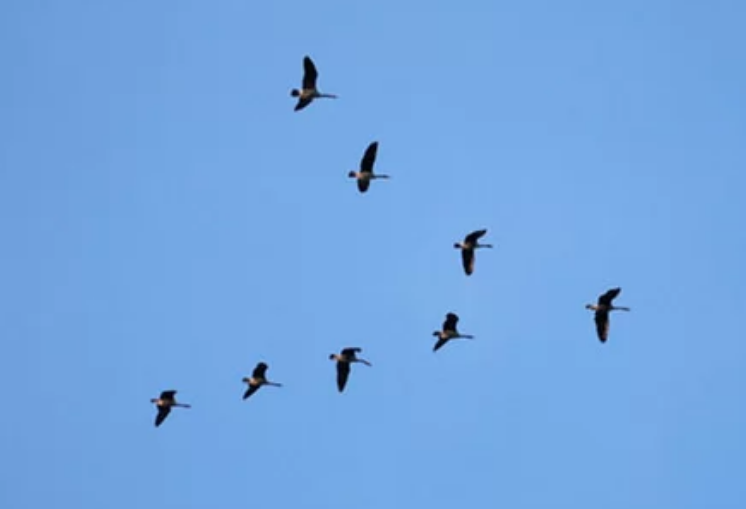
\includegraphics[width = \linewidth]{image/birdflock.png}
\caption{Flock of cranes}
\end{subfigure}
\begin{subfigure}{0.5\linewidth}
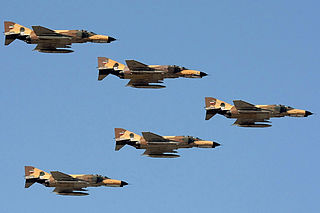
\includegraphics[width = \linewidth, trim=30 30 30 30,clip]{image/planeformation1.jpg}
\caption{Planes in formation}
\end{subfigure}
\caption{Formation Flying Analogy}
\label{fig:flock analogy}
\end{figure}

\subsection*{Applications}

The consumer base for UAVs comprises of entertainment industry (aerial photography), mapping industry (mosaicing of aerial images to create maps), mining industry (for creating 3D maps of the mines), precision agriculture and inspection of difficult to reach areas. However, the most important yet generally unknown users of UAVs are law enforcement and defense forces. The UAVs are very commonly used by law enforcement authorities for tasks like surveillance, crowd control and encroachment detection. In the recent years, use of UAVs by first responders going for aid in natural disaster scenario has increased considerably, highlighting their capabilities like never before.

The large and varied requirements of a disaster scenario makes it very difficult to design and develop an optimal and efficient UAV and hence each disaster scenario requires a different UAV. Also, the UAV developed to cover the whole affected area while providing ample situation's awareness tends be expensive, large and complex to operate and maintain. Failure of one such UAV may compromise the whole mission. As widely believed, multiple entities are always better than one. Thus, the author propose development of a testbed to help in implementing the popular algorithms developed for utilizing swarm behaviour in such life-altering situations. The ability to use many small vehicles instead of one large vehicle will increase efficiency, area coverage and situation's awareness while minimizing the risk of mission compromise.

Potential applications for a swarm of aerial robot are:

\begin{enumerate}
    \item \textbf{Search and Rescue Operations} around the globe have witnessed increasing use of UAVs as first responders acting as eyes and ears for the rescue teams scanning a wide area for possible survivors and delivering immediate medical supplies wherever required. Using multiple coordinated vehicles helps in sensor sharing and covering larger areas. Recent natural disasters like Cyclone Fani in Orissa and Chennai floods of 2018 were major grounds for use of UAVs for search and rescue missions.
    \item \textbf{Surveillance and Military Use} of UAV swarms includes aerial photography and videography and delivery of necessary payload or explosives. The presence of multiple vehicles with different capabilities allows for use of more sensors and varied payloads.
    \item \textbf{Entertainment} industry has witnessed the maximum usage of aerial swarms specially as a way to replace fireworks. The largest multi-rotor swarm demonstrations have been in the form of light shows by companies like Intel and Ehang.
    \item \textbf{Payload Transfer and Construction} applications of aerial swarms are under research at University of Pennsylvania and ETH Zurich.
\end{enumerate}

\subsection*{Features}
Various features commonly witnessed in robotic swarms can be classified as follows:
\begin{enumerate}
    \item \textbf{Aggregation} deals with spatially grouping all robots together in a region of the environment. It is used to get robots in a swarm sufficiently close together and can be used as a starting point for performing some additional tasks, such as communication with limited range. Aggregation near points of interest can be viewed as the first step of more complex tasks, such as collective transportation where objects of interest need to be transported by several robots. 
    \item \textbf{Pattern formation} is the deployment of robots into the environment forming a predefined geometric shape or pattern like a square, a circle, a line, a lattice etc. Pattern formation enables preserving communication range and overcoming environment limitations (e.g., passing a narrow passage by forming a chain).
    \item \textbf{Self-assembly} refers to the phenomenon of physical connection of robots to each other resulting in the formation of a particular structure. Self assembly is used to increase the pulling power of the robots, provide stability to the robot swarm while moving on rough terrains, form a connected structure to guide other swarm robots, assemble structures used to overcome holes that a single robot would fall into and to combine capabilities of heterogeneous robots. Self-assembly is studied in several large-scale research projects such as SWARM-BOTS, Symbrion, Swarmanoid , and Replicator.
    \item In\textbf{ swarm-guided} navigation robots of the swarm are navigated by other members of the swarm. Robots are not aware of their actual location or the location of the target. Instead, the swarm is guided by directions supplied by previously deployed robots forming a communication relay. Examples include robots forming a chain from a prey to the nest and indicating directions to other robots in a foraging task, navigation via exchanging navigation messages and flying robots navigating wheeled robots. 
\end{enumerate}

\subsection*{Advantages}
As stated earlier, the use of multiple robots in a coordinated manner has many advantages over use of a single, larger, bulkier and more expensive system capable of performing the same mission. Some of these advantages are listed below:

\begin{enumerate}
    \item Maximize Area Coverage \\Use of multiple vehicles increases the area coverage by dividing overall area into smaller cells to be covered by individual vehicles.
    \item Increased Reliability and Redundancy \\The loss of one vehicle doesn't sabotage the whole mission.
    \item Sensor and Payload Sharing \\The vehicles in an aerial swarm need not be identical to each other. This allows for use of a rich sensor suite and payload distributed among various vehicles.
    \item Reduction in size and Loss \\The size of an aerial robot grows rapidly with increase in payload weight. Thus, splitting of payload leads to smaller vehicles. The loss caused by failure of a smaller vehicle is much lesser.
    \item Parallel Execution of task saving time
\end{enumerate}

\subsection*{Disadvantages}
While robotic swarms increase the potential applications and use cases, they possess some limitations when compared to a single robot with similar capabilities. These limitations are as follows:
\begin{enumerate}
    \item Real time high bandwidth communication is required for swarm operations to exchange information between vehicles in the swarm and the ground control station.
    \item Increased operational complexity due to launching and planning multiple vehicles.
    \item Requirement of more human operators to deal with multiple vehicles.
\end{enumerate}

\section{Current State of the Art}
The state of the art UAV swarms implemented so far have been observed for academic research, entertainment or military applications only.

The United States of America and Chinese defence forces have successfully tested swarms of more than 50 fixed wing aircrafts in year 2015 and 2018 respectively. The details of these systems (centralized or decentralised, cooperative or time-varying trajectories etc) has not been provided in details. \\Companies like Intel and Ehang have demonstrated swarms of more than 1000 micro multirotors for the purpose of entertainment using time-varying trajectories and a centralised system. \\Scholars from various esteemed universities and institutes like Georgia Institute of Technology, University of Pennsylvania, ETH Zurich, National University of Singapore, Czech Technical University and École polytechnique fédérale de Lausanne (EPFL) are working in the field of swarm algorithm implementation. The GRASP lab headed by Dr. Vijay Kumar at University of Pennsylvania and the flying robotics club at ETH Zurich have set new benchmarks by creating algorithms that utilise the potential of swarms like never before and implementing them on small groups of quadcopters. Some of these systems are depicted in Fig. \ref{fig:currstate}
\begin{figure}[h]
\begin{subfigure}{0.5\textwidth}

\includegraphics[width=0.9\linewidth, height=5cm]{image/intel.png}
\caption{Intel Drone Show}
\end{subfigure}
\begin{subfigure}{0.5\textwidth}
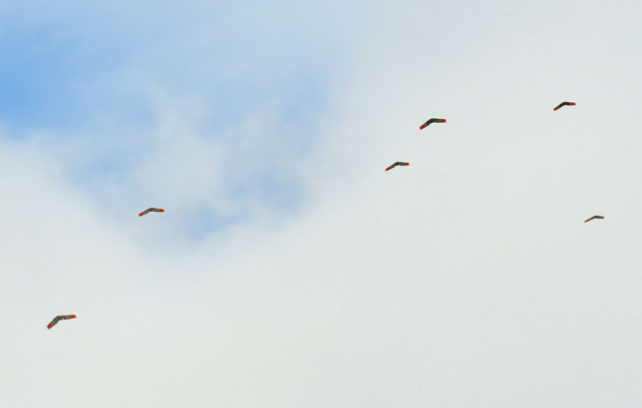
\includegraphics[width=0.9\linewidth, height=5cm]{image/navalps.png}
\caption{Naval Postgraduate School, US}
\end{subfigure}
 
 \begin{subfigure}{0.5\textwidth}
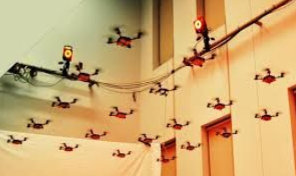
\includegraphics[width=0.9\linewidth, height=5cm]{image/upenn.png}
\caption{University of Pennsylvania}
\end{subfigure}
\begin{subfigure}{0.5\textwidth}
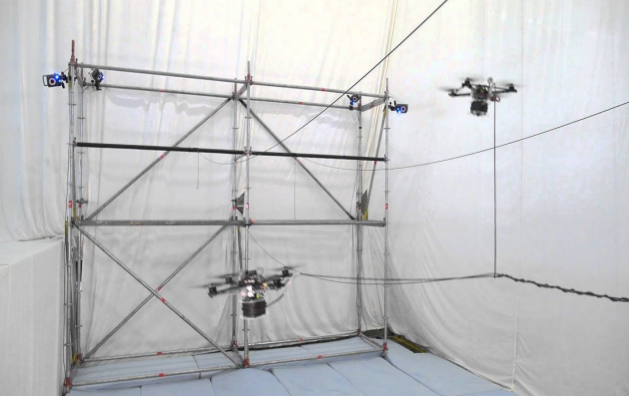
\includegraphics[width=0.9\linewidth, height=5cm]{image/ETH.png}
\caption{ETH Zurich}
\end{subfigure}

%\caption[Caption for LOF]{Physical Configurations of Fixed Robotic Manipulator\protect\footnotemark}
\caption{Current state of UAV Swarms}
\label{fig:currstate}
\end{figure}
%\footnotetext{Courtesy of https://nptel.ac.in/courses/112103174/module7/lec5/3.html}

\section{Challenges}
Development and implementation of aerial swarms is still under research and faces many challenges, some of these are:
\begin{enumerate}
    \item Lack of reliable Communication system
    \item Precise Localisation
    \item High Cost
\end{enumerate}
\end{spacing}